\documentclass[12pt]{article}

\usepackage{amsmath}    % need for subequations
\usepackage{graphicx}   % need for figures
\usepackage{verbatim}   % useful for program listings
\usepackage{color}      % use if color is used in text
\usepackage{subfigure}  % use for side-by-side figures
\usepackage{hyperref}   % use for hypertext links, including those to external documents and URLs
\usepackage{tikz}
\usepackage{pgfplots}

\begin{document}
\begin{figure}
\centering
% Created by tikzDevice version 0.7.0 on 2015-04-28 12:37:09
% !TEX encoding = UTF-8 Unicode
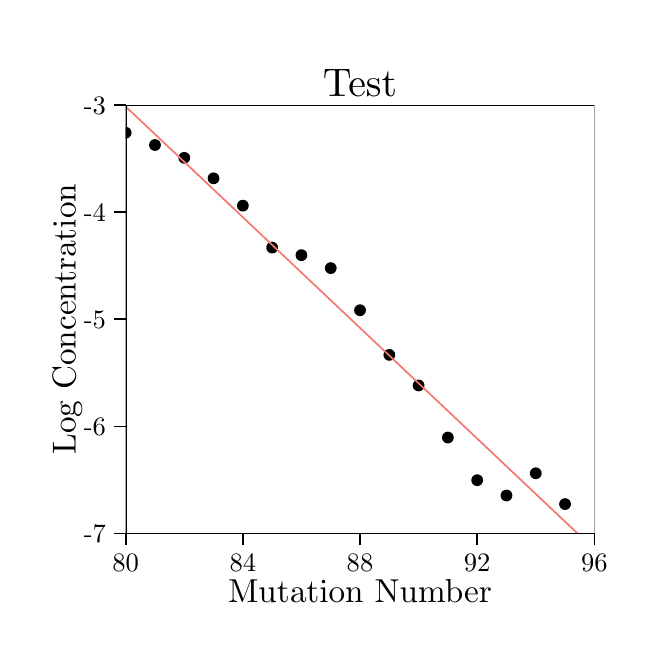
\begin{tikzpicture}[x=1pt,y=1pt]
\definecolor[named]{fillColor}{rgb}{1.00,1.00,1.00}
\path[use as bounding box,fill=fillColor,fill opacity=0.00] (0,0) rectangle (216.81,216.81);
\begin{scope}
\path[clip] (  0.00,  0.00) rectangle (216.81,216.81);
\definecolor[named]{drawColor}{rgb}{1.00,1.00,1.00}
\definecolor[named]{fillColor}{rgb}{1.00,1.00,1.00}

\path[draw=drawColor,line width= 0.6pt,line join=round,line cap=round,fill=fillColor] (  0.00,  0.00) rectangle (216.81,216.81);
\end{scope}
\begin{scope}
\path[clip] ( 35.42, 34.03) rectangle (204.76,188.82);
\definecolor[named]{fillColor}{rgb}{1.00,1.00,1.00}

\path[fill=fillColor] ( 35.42, 34.03) rectangle (204.76,188.82);
\definecolor[named]{fillColor}{rgb}{0.00,0.00,0.00}

\path[fill=fillColor] ( 35.42,178.84) circle (  2.13);

\path[fill=fillColor] ( 46.00,174.41) circle (  2.13);

\path[fill=fillColor] ( 56.59,169.78) circle (  2.13);

\path[fill=fillColor] ( 67.17,162.37) circle (  2.13);

\path[fill=fillColor] ( 77.76,152.49) circle (  2.13);

\path[fill=fillColor] ( 88.34,137.35) circle (  2.13);

\path[fill=fillColor] ( 98.92,134.61) circle (  2.13);

\path[fill=fillColor] (109.51,129.93) circle (  2.13);

\path[fill=fillColor] (120.09,114.71) circle (  2.13);

\path[fill=fillColor] (130.68, 98.57) circle (  2.13);

\path[fill=fillColor] (141.26, 87.53) circle (  2.13);

\path[fill=fillColor] (151.84, 68.70) circle (  2.13);

\path[fill=fillColor] (162.43, 53.29) circle (  2.13);

\path[fill=fillColor] (173.01, 47.76) circle (  2.13);

\path[fill=fillColor] (183.60, 55.79) circle (  2.13);

\path[fill=fillColor] (194.18, 44.66) circle (  2.13);
\definecolor[named]{drawColor}{rgb}{0.97,0.46,0.43}
\definecolor[named]{fillColor}{rgb}{0.97,0.46,0.43}

\path[draw=drawColor,line width= 0.6pt,line join=round,fill=fillColor] ( 35.42,188.31) -- (204.76, 28.32);
\definecolor[named]{drawColor}{rgb}{0.00,0.00,0.00}

\path[draw=drawColor,line width= 0.6pt,line join=round,line cap=round] ( 35.42, 34.03) rectangle (204.76,188.82);
\end{scope}
\begin{scope}
\path[clip] (  0.00,  0.00) rectangle (216.81,216.81);
\definecolor[named]{drawColor}{rgb}{0.00,0.00,0.00}

\node[text=drawColor,anchor=base east,inner sep=0pt, outer sep=0pt, scale=  0.96] at ( 28.31, 30.73) {-7};

\node[text=drawColor,anchor=base east,inner sep=0pt, outer sep=0pt, scale=  0.96] at ( 28.31, 69.43) {-6};

\node[text=drawColor,anchor=base east,inner sep=0pt, outer sep=0pt, scale=  0.96] at ( 28.31,108.12) {-5};

\node[text=drawColor,anchor=base east,inner sep=0pt, outer sep=0pt, scale=  0.96] at ( 28.31,146.82) {-4};

\node[text=drawColor,anchor=base east,inner sep=0pt, outer sep=0pt, scale=  0.96] at ( 28.31,185.52) {-3};
\end{scope}
\begin{scope}
\path[clip] (  0.00,  0.00) rectangle (216.81,216.81);
\definecolor[named]{drawColor}{rgb}{0.00,0.00,0.00}

\path[draw=drawColor,line width= 0.6pt,line join=round] ( 31.15, 34.03) --
	( 35.42, 34.03);

\path[draw=drawColor,line width= 0.6pt,line join=round] ( 31.15, 72.73) --
	( 35.42, 72.73);

\path[draw=drawColor,line width= 0.6pt,line join=round] ( 31.15,111.43) --
	( 35.42,111.43);

\path[draw=drawColor,line width= 0.6pt,line join=round] ( 31.15,150.13) --
	( 35.42,150.13);

\path[draw=drawColor,line width= 0.6pt,line join=round] ( 31.15,188.82) --
	( 35.42,188.82);
\end{scope}
\begin{scope}
\path[clip] (  0.00,  0.00) rectangle (216.81,216.81);
\definecolor[named]{drawColor}{rgb}{0.00,0.00,0.00}

\path[draw=drawColor,line width= 0.6pt,line join=round] ( 35.42, 29.77) --
	( 35.42, 34.03);

\path[draw=drawColor,line width= 0.6pt,line join=round] ( 77.76, 29.77) --
	( 77.76, 34.03);

\path[draw=drawColor,line width= 0.6pt,line join=round] (120.09, 29.77) --
	(120.09, 34.03);

\path[draw=drawColor,line width= 0.6pt,line join=round] (162.43, 29.77) --
	(162.43, 34.03);

\path[draw=drawColor,line width= 0.6pt,line join=round] (204.76, 29.77) --
	(204.76, 34.03);
\end{scope}
\begin{scope}
\path[clip] (  0.00,  0.00) rectangle (216.81,216.81);
\definecolor[named]{drawColor}{rgb}{0.00,0.00,0.00}

\node[text=drawColor,anchor=base,inner sep=0pt, outer sep=0pt, scale=  0.96] at ( 35.42, 20.31) {80};

\node[text=drawColor,anchor=base,inner sep=0pt, outer sep=0pt, scale=  0.96] at ( 77.76, 20.31) {84};

\node[text=drawColor,anchor=base,inner sep=0pt, outer sep=0pt, scale=  0.96] at (120.09, 20.31) {88};

\node[text=drawColor,anchor=base,inner sep=0pt, outer sep=0pt, scale=  0.96] at (162.43, 20.31) {92};

\node[text=drawColor,anchor=base,inner sep=0pt, outer sep=0pt, scale=  0.96] at (204.76, 20.31) {96};
\end{scope}
\begin{scope}
\path[clip] (  0.00,  0.00) rectangle (216.81,216.81);
\definecolor[named]{drawColor}{rgb}{0.00,0.00,0.00}

\node[text=drawColor,anchor=base,inner sep=0pt, outer sep=0pt, scale=  1.20] at (120.09,  9.03) {Mutation Number};
\end{scope}
\begin{scope}
\path[clip] (  0.00,  0.00) rectangle (216.81,216.81);
\definecolor[named]{drawColor}{rgb}{0.00,0.00,0.00}

\node[text=drawColor,rotate= 90.00,anchor=base,inner sep=0pt, outer sep=0pt, scale=  1.20] at ( 17.30,111.43) {Log Concentration};
\end{scope}
\begin{scope}
\path[clip] (  0.00,  0.00) rectangle (216.81,216.81);
\definecolor[named]{drawColor}{rgb}{0.00,0.00,0.00}

\node[text=drawColor,anchor=base,inner sep=0pt, outer sep=0pt, scale=  1.44] at (120.09,191.84) {Test};
\end{scope}
\end{tikzpicture}

\end{figure}
\begin{figure}
\centering
% Created by tikzDevice version 0.7.0 on 2015-04-30 10:54:43
% !TEX encoding = UTF-8 Unicode
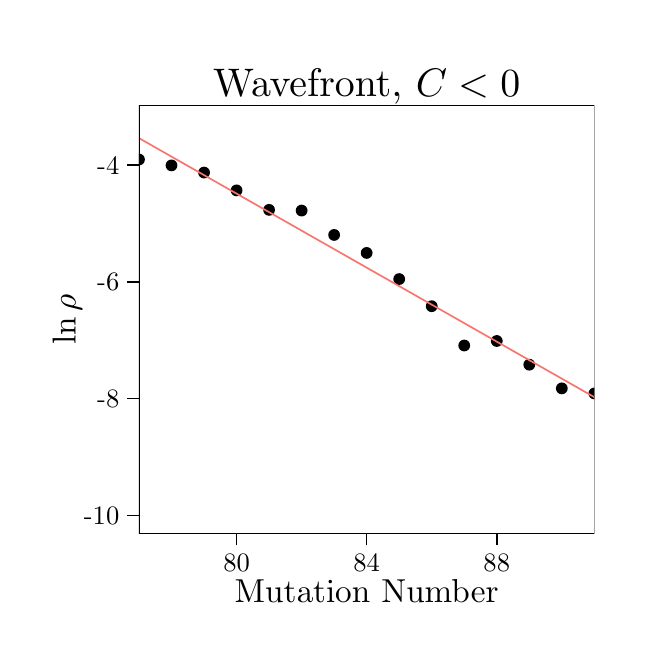
\begin{tikzpicture}[x=1pt,y=1pt]
\definecolor[named]{fillColor}{rgb}{1.00,1.00,1.00}
\path[use as bounding box,fill=fillColor,fill opacity=0.00] (0,0) rectangle (216.81,216.81);
\begin{scope}
\path[clip] (  0.00,  0.00) rectangle (216.81,216.81);
\definecolor[named]{drawColor}{rgb}{1.00,1.00,1.00}
\definecolor[named]{fillColor}{rgb}{1.00,1.00,1.00}

\path[draw=drawColor,line width= 0.6pt,line join=round,line cap=round,fill=fillColor] (  0.00,  0.00) rectangle (216.81,216.81);
\end{scope}
\begin{scope}
\path[clip] ( 40.22, 34.03) rectangle (204.76,188.82);
\definecolor[named]{fillColor}{rgb}{1.00,1.00,1.00}

\path[fill=fillColor] ( 40.22, 34.03) rectangle (204.76,188.82);
\definecolor[named]{fillColor}{rgb}{0.00,0.00,0.00}

\path[fill=fillColor] ( 40.22,169.17) circle (  2.13);

\path[fill=fillColor] ( 51.97,167.04) circle (  2.13);

\path[fill=fillColor] ( 63.73,164.45) circle (  2.13);

\path[fill=fillColor] ( 75.48,158.01) circle (  2.13);

\path[fill=fillColor] ( 87.23,150.97) circle (  2.13);

\path[fill=fillColor] ( 98.99,150.72) circle (  2.13);

\path[fill=fillColor] (110.74,141.91) circle (  2.13);

\path[fill=fillColor] (122.49,135.41) circle (  2.13);

\path[fill=fillColor] (134.25,125.97) circle (  2.13);

\path[fill=fillColor] (146.00,116.16) circle (  2.13);

\path[fill=fillColor] (157.75,101.96) circle (  2.13);

\path[fill=fillColor] (169.51,103.59) circle (  2.13);

\path[fill=fillColor] (181.26, 95.03) circle (  2.13);

\path[fill=fillColor] (193.01, 86.47) circle (  2.13);

\path[fill=fillColor] (204.76, 84.64) circle (  2.13);
\definecolor[named]{drawColor}{rgb}{0.97,0.46,0.43}
\definecolor[named]{fillColor}{rgb}{0.97,0.46,0.43}

\path[draw=drawColor,line width= 0.6pt,line join=round,fill=fillColor] ( 40.22,176.90) -- (204.76, 83.30);
\definecolor[named]{drawColor}{rgb}{0.00,0.00,0.00}

\path[draw=drawColor,line width= 0.6pt,line join=round,line cap=round] ( 40.22, 34.03) rectangle (204.76,188.82);
\end{scope}
\begin{scope}
\path[clip] (  0.00,  0.00) rectangle (216.81,216.81);
\definecolor[named]{drawColor}{rgb}{0.00,0.00,0.00}

\node[text=drawColor,anchor=base east,inner sep=0pt, outer sep=0pt, scale=  0.96] at ( 33.11, 37.25) {-10};

\node[text=drawColor,anchor=base east,inner sep=0pt, outer sep=0pt, scale=  0.96] at ( 33.11, 79.45) {-8};

\node[text=drawColor,anchor=base east,inner sep=0pt, outer sep=0pt, scale=  0.96] at ( 33.11,121.66) {-6};

\node[text=drawColor,anchor=base east,inner sep=0pt, outer sep=0pt, scale=  0.96] at ( 33.11,163.87) {-4};
\end{scope}
\begin{scope}
\path[clip] (  0.00,  0.00) rectangle (216.81,216.81);
\definecolor[named]{drawColor}{rgb}{0.00,0.00,0.00}

\path[draw=drawColor,line width= 0.6pt,line join=round] ( 35.95, 40.55) --
	( 40.22, 40.55);

\path[draw=drawColor,line width= 0.6pt,line join=round] ( 35.95, 82.76) --
	( 40.22, 82.76);

\path[draw=drawColor,line width= 0.6pt,line join=round] ( 35.95,124.97) --
	( 40.22,124.97);

\path[draw=drawColor,line width= 0.6pt,line join=round] ( 35.95,167.17) --
	( 40.22,167.17);
\end{scope}
\begin{scope}
\path[clip] (  0.00,  0.00) rectangle (216.81,216.81);
\definecolor[named]{drawColor}{rgb}{0.00,0.00,0.00}

\path[draw=drawColor,line width= 0.6pt,line join=round] ( 75.48, 29.77) --
	( 75.48, 34.03);

\path[draw=drawColor,line width= 0.6pt,line join=round] (122.49, 29.77) --
	(122.49, 34.03);

\path[draw=drawColor,line width= 0.6pt,line join=round] (169.51, 29.77) --
	(169.51, 34.03);
\end{scope}
\begin{scope}
\path[clip] (  0.00,  0.00) rectangle (216.81,216.81);
\definecolor[named]{drawColor}{rgb}{0.00,0.00,0.00}

\node[text=drawColor,anchor=base,inner sep=0pt, outer sep=0pt, scale=  0.96] at ( 75.48, 20.31) {80};

\node[text=drawColor,anchor=base,inner sep=0pt, outer sep=0pt, scale=  0.96] at (122.49, 20.31) {84};

\node[text=drawColor,anchor=base,inner sep=0pt, outer sep=0pt, scale=  0.96] at (169.51, 20.31) {88};
\end{scope}
\begin{scope}
\path[clip] (  0.00,  0.00) rectangle (216.81,216.81);
\definecolor[named]{drawColor}{rgb}{0.00,0.00,0.00}

\node[text=drawColor,anchor=base,inner sep=0pt, outer sep=0pt, scale=  1.20] at (122.49,  9.03) {Mutation Number};
\end{scope}
\begin{scope}
\path[clip] (  0.00,  0.00) rectangle (216.81,216.81);
\definecolor[named]{drawColor}{rgb}{0.00,0.00,0.00}

\node[text=drawColor,rotate= 90.00,anchor=base,inner sep=0pt, outer sep=0pt, scale=  1.20] at ( 17.30,111.43) {$\ln \rho$};
\end{scope}
\begin{scope}
\path[clip] (  0.00,  0.00) rectangle (216.81,216.81);
\definecolor[named]{drawColor}{rgb}{0.00,0.00,0.00}

\node[text=drawColor,anchor=base,inner sep=0pt, outer sep=0pt, scale=  1.44] at (122.49,191.84) {Wavefront, $C<0$};
\end{scope}
\end{tikzpicture}

\end{figure}
\begin{figure}
\centering
% Created by tikzDevice version 0.7.0 on 2015-04-30 10:54:44
% !TEX encoding = UTF-8 Unicode
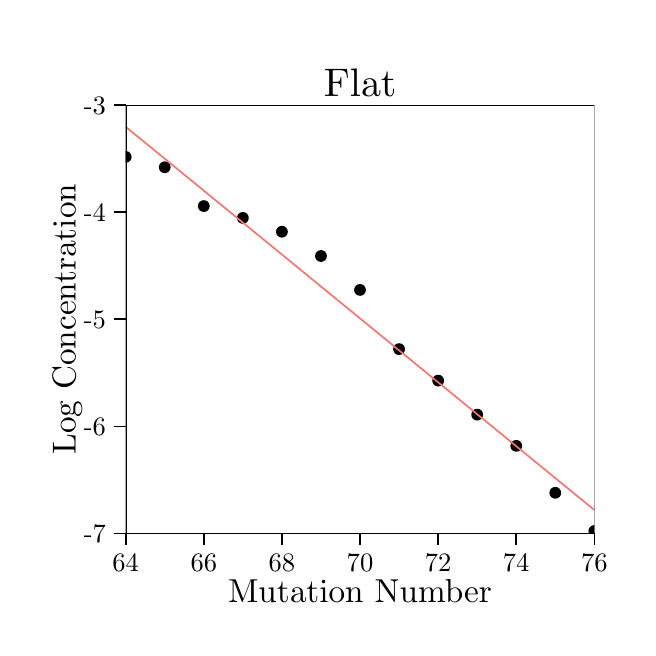
\begin{tikzpicture}[x=1pt,y=1pt]
\definecolor[named]{fillColor}{rgb}{1.00,1.00,1.00}
\path[use as bounding box,fill=fillColor,fill opacity=0.00] (0,0) rectangle (216.81,216.81);
\begin{scope}
\path[clip] (  0.00,  0.00) rectangle (216.81,216.81);
\definecolor[named]{drawColor}{rgb}{1.00,1.00,1.00}
\definecolor[named]{fillColor}{rgb}{1.00,1.00,1.00}

\path[draw=drawColor,line width= 0.6pt,line join=round,line cap=round,fill=fillColor] (  0.00,  0.00) rectangle (216.81,216.81);
\end{scope}
\begin{scope}
\path[clip] ( 35.42, 34.03) rectangle (204.76,188.82);
\definecolor[named]{fillColor}{rgb}{1.00,1.00,1.00}

\path[fill=fillColor] ( 35.42, 34.03) rectangle (204.76,188.82);
\definecolor[named]{fillColor}{rgb}{0.00,0.00,0.00}

\path[fill=fillColor] ( 35.42,170.11) circle (  2.13);

\path[fill=fillColor] ( 49.53,166.37) circle (  2.13);

\path[fill=fillColor] ( 63.64,152.35) circle (  2.13);

\path[fill=fillColor] ( 77.76,148.07) circle (  2.13);

\path[fill=fillColor] ( 91.87,143.08) circle (  2.13);

\path[fill=fillColor] (105.98,134.30) circle (  2.13);

\path[fill=fillColor] (120.09,122.05) circle (  2.13);

\path[fill=fillColor] (134.20,100.65) circle (  2.13);

\path[fill=fillColor] (148.32, 89.27) circle (  2.13);

\path[fill=fillColor] (162.43, 76.98) circle (  2.13);

\path[fill=fillColor] (176.54, 65.70) circle (  2.13);

\path[fill=fillColor] (190.65, 48.74) circle (  2.13);

\path[fill=fillColor] (204.76, 34.93) circle (  2.13);
\definecolor[named]{drawColor}{rgb}{0.97,0.46,0.43}
\definecolor[named]{fillColor}{rgb}{0.97,0.46,0.43}

\path[draw=drawColor,line width= 0.6pt,line join=round,fill=fillColor] ( 35.42,180.98) -- (204.76, 42.50);
\definecolor[named]{drawColor}{rgb}{0.00,0.00,0.00}

\path[draw=drawColor,line width= 0.6pt,line join=round,line cap=round] ( 35.42, 34.03) rectangle (204.76,188.82);
\end{scope}
\begin{scope}
\path[clip] (  0.00,  0.00) rectangle (216.81,216.81);
\definecolor[named]{drawColor}{rgb}{0.00,0.00,0.00}

\node[text=drawColor,anchor=base east,inner sep=0pt, outer sep=0pt, scale=  0.96] at ( 28.31, 30.73) {-7};

\node[text=drawColor,anchor=base east,inner sep=0pt, outer sep=0pt, scale=  0.96] at ( 28.31, 69.43) {-6};

\node[text=drawColor,anchor=base east,inner sep=0pt, outer sep=0pt, scale=  0.96] at ( 28.31,108.12) {-5};

\node[text=drawColor,anchor=base east,inner sep=0pt, outer sep=0pt, scale=  0.96] at ( 28.31,146.82) {-4};

\node[text=drawColor,anchor=base east,inner sep=0pt, outer sep=0pt, scale=  0.96] at ( 28.31,185.52) {-3};
\end{scope}
\begin{scope}
\path[clip] (  0.00,  0.00) rectangle (216.81,216.81);
\definecolor[named]{drawColor}{rgb}{0.00,0.00,0.00}

\path[draw=drawColor,line width= 0.6pt,line join=round] ( 31.15, 34.03) --
	( 35.42, 34.03);

\path[draw=drawColor,line width= 0.6pt,line join=round] ( 31.15, 72.73) --
	( 35.42, 72.73);

\path[draw=drawColor,line width= 0.6pt,line join=round] ( 31.15,111.43) --
	( 35.42,111.43);

\path[draw=drawColor,line width= 0.6pt,line join=round] ( 31.15,150.13) --
	( 35.42,150.13);

\path[draw=drawColor,line width= 0.6pt,line join=round] ( 31.15,188.82) --
	( 35.42,188.82);
\end{scope}
\begin{scope}
\path[clip] (  0.00,  0.00) rectangle (216.81,216.81);
\definecolor[named]{drawColor}{rgb}{0.00,0.00,0.00}

\path[draw=drawColor,line width= 0.6pt,line join=round] ( 35.42, 29.77) --
	( 35.42, 34.03);

\path[draw=drawColor,line width= 0.6pt,line join=round] ( 63.64, 29.77) --
	( 63.64, 34.03);

\path[draw=drawColor,line width= 0.6pt,line join=round] ( 91.87, 29.77) --
	( 91.87, 34.03);

\path[draw=drawColor,line width= 0.6pt,line join=round] (120.09, 29.77) --
	(120.09, 34.03);

\path[draw=drawColor,line width= 0.6pt,line join=round] (148.32, 29.77) --
	(148.32, 34.03);

\path[draw=drawColor,line width= 0.6pt,line join=round] (176.54, 29.77) --
	(176.54, 34.03);

\path[draw=drawColor,line width= 0.6pt,line join=round] (204.76, 29.77) --
	(204.76, 34.03);
\end{scope}
\begin{scope}
\path[clip] (  0.00,  0.00) rectangle (216.81,216.81);
\definecolor[named]{drawColor}{rgb}{0.00,0.00,0.00}

\node[text=drawColor,anchor=base,inner sep=0pt, outer sep=0pt, scale=  0.96] at ( 35.42, 20.31) {64};

\node[text=drawColor,anchor=base,inner sep=0pt, outer sep=0pt, scale=  0.96] at ( 63.64, 20.31) {66};

\node[text=drawColor,anchor=base,inner sep=0pt, outer sep=0pt, scale=  0.96] at ( 91.87, 20.31) {68};

\node[text=drawColor,anchor=base,inner sep=0pt, outer sep=0pt, scale=  0.96] at (120.09, 20.31) {70};

\node[text=drawColor,anchor=base,inner sep=0pt, outer sep=0pt, scale=  0.96] at (148.32, 20.31) {72};

\node[text=drawColor,anchor=base,inner sep=0pt, outer sep=0pt, scale=  0.96] at (176.54, 20.31) {74};

\node[text=drawColor,anchor=base,inner sep=0pt, outer sep=0pt, scale=  0.96] at (204.76, 20.31) {76};
\end{scope}
\begin{scope}
\path[clip] (  0.00,  0.00) rectangle (216.81,216.81);
\definecolor[named]{drawColor}{rgb}{0.00,0.00,0.00}

\node[text=drawColor,anchor=base,inner sep=0pt, outer sep=0pt, scale=  1.20] at (120.09,  9.03) {Mutation Number};
\end{scope}
\begin{scope}
\path[clip] (  0.00,  0.00) rectangle (216.81,216.81);
\definecolor[named]{drawColor}{rgb}{0.00,0.00,0.00}

\node[text=drawColor,rotate= 90.00,anchor=base,inner sep=0pt, outer sep=0pt, scale=  1.20] at ( 17.30,111.43) {Log Concentration};
\end{scope}
\begin{scope}
\path[clip] (  0.00,  0.00) rectangle (216.81,216.81);
\definecolor[named]{drawColor}{rgb}{0.00,0.00,0.00}

\node[text=drawColor,anchor=base,inner sep=0pt, outer sep=0pt, scale=  1.44] at (120.09,191.84) {Flat};
\end{scope}
\end{tikzpicture}

\end{figure}
\begin{figure}
\centering
% Created by tikzDevice version 0.7.0 on 2015-04-30 12:06:24
% !TEX encoding = UTF-8 Unicode
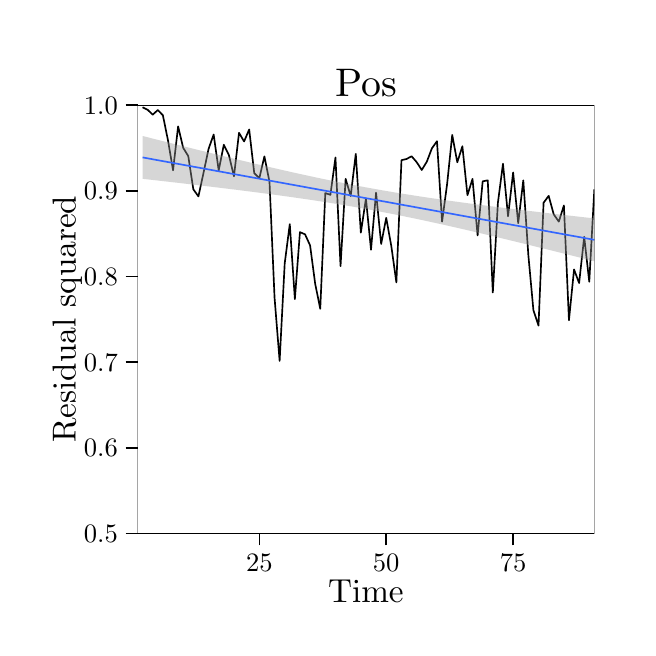
\begin{tikzpicture}[x=1pt,y=1pt]
\definecolor[named]{fillColor}{rgb}{1.00,1.00,1.00}
\path[use as bounding box,fill=fillColor,fill opacity=0.00] (0,0) rectangle (216.81,216.81);
\begin{scope}
\path[clip] (  0.00,  0.00) rectangle (216.81,216.81);
\definecolor[named]{drawColor}{rgb}{1.00,1.00,1.00}
\definecolor[named]{fillColor}{rgb}{1.00,1.00,1.00}

\path[draw=drawColor,line width= 0.6pt,line join=round,line cap=round,fill=fillColor] ( -0.00,  0.00) rectangle (216.81,216.81);
\end{scope}
\begin{scope}
\path[clip] ( 39.69, 34.03) rectangle (204.76,188.82);
\definecolor[named]{fillColor}{rgb}{1.00,1.00,1.00}

\path[fill=fillColor] ( 39.69, 34.03) rectangle (204.76,188.82);
\definecolor[named]{drawColor}{rgb}{0.00,0.00,0.00}

\path[draw=drawColor,line width= 0.6pt,line join=round] ( 41.52,188.04) --
	( 43.35,187.14) --
	( 45.19,185.37) --
	( 47.02,187.05) --
	( 48.86,185.15) --
	( 50.69,176.14) --
	( 52.53,165.27) --
	( 54.36,181.12) --
	( 56.19,173.40) --
	( 58.03,170.40) --
	( 59.86,158.39) --
	( 61.70,155.85) --
	( 63.53,164.30) --
	( 65.37,173.01) --
	( 67.20,178.19) --
	( 69.03,165.21) --
	( 70.87,174.50) --
	( 72.70,170.79) --
	( 74.54,163.11) --
	( 76.37,178.81) --
	( 78.20,175.68) --
	( 80.04,180.03) --
	( 81.87,164.25) --
	( 83.71,162.42) --
	( 85.54,170.29) --
	( 87.38,161.10) --
	( 89.21,119.21) --
	( 91.04, 96.38) --
	( 92.88,131.64) --
	( 94.71,145.82) --
	( 96.55,118.74) --
	( 98.38,142.92) --
	(100.22,142.14) --
	(102.05,138.13) --
	(103.88,124.33) --
	(105.72,115.20) --
	(107.55,157.05) --
	(109.39,156.41) --
	(111.22,169.90) --
	(113.05,130.63) --
	(114.89,162.19) --
	(116.72,155.96) --
	(118.56,171.21) --
	(120.39,142.73) --
	(122.23,155.04) --
	(124.06,136.58) --
	(125.89,157.17) --
	(127.73,138.64) --
	(129.56,148.08) --
	(131.40,137.87) --
	(133.23,124.74) --
	(135.07,168.93) --
	(136.90,169.36) --
	(138.73,170.34) --
	(140.57,168.20) --
	(142.40,165.39) --
	(144.24,168.40) --
	(146.07,173.21) --
	(147.90,175.78) --
	(149.74,146.71) --
	(151.57,160.36) --
	(153.41,178.06) --
	(155.24,168.16) --
	(157.08,173.95) --
	(158.91,156.28) --
	(160.74,162.18) --
	(162.58,141.72) --
	(164.41,161.28) --
	(166.25,161.65) --
	(168.08,121.12) --
	(169.92,153.57) --
	(171.75,167.62) --
	(173.58,148.65) --
	(175.42,164.48) --
	(177.25,146.16) --
	(179.09,161.63) --
	(180.92,134.58) --
	(182.75,114.67) --
	(184.59,109.14) --
	(186.42,153.54) --
	(188.26,156.04) --
	(190.09,149.34) --
	(191.93,146.72) --
	(193.76,152.55) --
	(195.59,111.10) --
	(197.43,129.43) --
	(199.26,124.53) --
	(201.10,141.23) --
	(202.93,124.96) --
	(204.76,158.36);
\definecolor[named]{fillColor}{rgb}{0.60,0.60,0.60}

\path[fill=fillColor,fill opacity=0.40] ( 41.52,177.66) --
	( 43.59,177.14) --
	( 45.65,176.62) --
	( 47.72,176.09) --
	( 49.79,175.58) --
	( 51.85,175.06) --
	( 53.92,174.54) --
	( 55.99,174.02) --
	( 58.05,173.51) --
	( 60.12,173.00) --
	( 62.18,172.49) --
	( 64.25,171.98) --
	( 66.32,171.47) --
	( 68.38,170.96) --
	( 70.45,170.46) --
	( 72.52,169.96) --
	( 74.58,169.46) --
	( 76.65,168.96) --
	( 78.72,168.47) --
	( 80.78,167.98) --
	( 82.85,167.49) --
	( 84.91,167.01) --
	( 86.98,166.53) --
	( 89.05,166.05) --
	( 91.11,165.58) --
	( 93.18,165.11) --
	( 95.25,164.64) --
	( 97.31,164.18) --
	( 99.38,163.73) --
	(101.45,163.28) --
	(103.51,162.83) --
	(105.58,162.39) --
	(107.65,161.96) --
	(109.71,161.54) --
	(111.78,161.12) --
	(113.84,160.70) --
	(115.91,160.30) --
	(117.98,159.90) --
	(120.04,159.51) --
	(122.11,159.12) --
	(124.18,158.75) --
	(126.24,158.38) --
	(128.31,158.01) --
	(130.38,157.66) --
	(132.44,157.31) --
	(134.51,156.97) --
	(136.57,156.64) --
	(138.64,156.31) --
	(140.71,155.99) --
	(142.77,155.67) --
	(144.84,155.36) --
	(146.91,155.06) --
	(148.97,154.76) --
	(151.04,154.46) --
	(153.11,154.17) --
	(155.17,153.89) --
	(157.24,153.61) --
	(159.30,153.33) --
	(161.37,153.06) --
	(163.44,152.79) --
	(165.50,152.52) --
	(167.57,152.26) --
	(169.64,152.00) --
	(171.70,151.74) --
	(173.77,151.49) --
	(175.84,151.24) --
	(177.90,150.99) --
	(179.97,150.74) --
	(182.03,150.49) --
	(184.10,150.25) --
	(186.17,150.00) --
	(188.23,149.76) --
	(190.30,149.52) --
	(192.37,149.28) --
	(194.43,149.05) --
	(196.50,148.81) --
	(198.57,148.58) --
	(200.63,148.34) --
	(202.70,148.11) --
	(204.76,147.88) --
	(204.76,132.41) --
	(202.70,132.93) --
	(200.63,133.45) --
	(198.57,133.98) --
	(196.50,134.49) --
	(194.43,135.01) --
	(192.37,135.53) --
	(190.30,136.05) --
	(188.23,136.56) --
	(186.17,137.07) --
	(184.10,137.58) --
	(182.03,138.09) --
	(179.97,138.60) --
	(177.90,139.11) --
	(175.84,139.61) --
	(173.77,140.11) --
	(171.70,140.61) --
	(169.64,141.11) --
	(167.57,141.60) --
	(165.50,142.09) --
	(163.44,142.58) --
	(161.37,143.06) --
	(159.30,143.54) --
	(157.24,144.02) --
	(155.17,144.49) --
	(153.11,144.96) --
	(151.04,145.43) --
	(148.97,145.89) --
	(146.91,146.34) --
	(144.84,146.79) --
	(142.77,147.24) --
	(140.71,147.67) --
	(138.64,148.11) --
	(136.57,148.53) --
	(134.51,148.95) --
	(132.44,149.37) --
	(130.38,149.77) --
	(128.31,150.17) --
	(126.24,150.56) --
	(124.18,150.95) --
	(122.11,151.32) --
	(120.04,151.69) --
	(117.98,152.06) --
	(115.91,152.41) --
	(113.84,152.76) --
	(111.78,153.10) --
	(109.71,153.43) --
	(107.65,153.76) --
	(105.58,154.08) --
	(103.51,154.40) --
	(101.45,154.71) --
	( 99.38,155.01) --
	( 97.31,155.31) --
	( 95.25,155.61) --
	( 93.18,155.89) --
	( 91.11,156.18) --
	( 89.05,156.46) --
	( 86.98,156.74) --
	( 84.91,157.01) --
	( 82.85,157.28) --
	( 80.78,157.55) --
	( 78.72,157.81) --
	( 76.65,158.07) --
	( 74.58,158.33) --
	( 72.52,158.58) --
	( 70.45,158.83) --
	( 68.38,159.08) --
	( 66.32,159.33) --
	( 64.25,159.58) --
	( 62.18,159.82) --
	( 60.12,160.07) --
	( 58.05,160.31) --
	( 55.99,160.55) --
	( 53.92,160.79) --
	( 51.85,161.02) --
	( 49.79,161.26) --
	( 47.72,161.49) --
	( 45.65,161.73) --
	( 43.59,161.96) --
	( 41.52,162.19) --
	cycle;
\definecolor[named]{drawColor}{rgb}{0.20,0.40,1.00}

\path[draw=drawColor,line width= 0.6pt,line join=round] ( 41.52,169.93) --
	( 43.59,169.55) --
	( 45.65,169.17) --
	( 47.72,168.79) --
	( 49.79,168.42) --
	( 51.85,168.04) --
	( 53.92,167.66) --
	( 55.99,167.29) --
	( 58.05,166.91) --
	( 60.12,166.53) --
	( 62.18,166.16) --
	( 64.25,165.78) --
	( 66.32,165.40) --
	( 68.38,165.02) --
	( 70.45,164.65) --
	( 72.52,164.27) --
	( 74.58,163.89) --
	( 76.65,163.52) --
	( 78.72,163.14) --
	( 80.78,162.76) --
	( 82.85,162.39) --
	( 84.91,162.01) --
	( 86.98,161.63) --
	( 89.05,161.25) --
	( 91.11,160.88) --
	( 93.18,160.50) --
	( 95.25,160.12) --
	( 97.31,159.75) --
	( 99.38,159.37) --
	(101.45,158.99) --
	(103.51,158.62) --
	(105.58,158.24) --
	(107.65,157.86) --
	(109.71,157.49) --
	(111.78,157.11) --
	(113.84,156.73) --
	(115.91,156.35) --
	(117.98,155.98) --
	(120.04,155.60) --
	(122.11,155.22) --
	(124.18,154.85) --
	(126.24,154.47) --
	(128.31,154.09) --
	(130.38,153.72) --
	(132.44,153.34) --
	(134.51,152.96) --
	(136.57,152.58) --
	(138.64,152.21) --
	(140.71,151.83) --
	(142.77,151.45) --
	(144.84,151.08) --
	(146.91,150.70) --
	(148.97,150.32) --
	(151.04,149.95) --
	(153.11,149.57) --
	(155.17,149.19) --
	(157.24,148.81) --
	(159.30,148.44) --
	(161.37,148.06) --
	(163.44,147.68) --
	(165.50,147.31) --
	(167.57,146.93) --
	(169.64,146.55) --
	(171.70,146.18) --
	(173.77,145.80) --
	(175.84,145.42) --
	(177.90,145.05) --
	(179.97,144.67) --
	(182.03,144.29) --
	(184.10,143.91) --
	(186.17,143.54) --
	(188.23,143.16) --
	(190.30,142.78) --
	(192.37,142.41) --
	(194.43,142.03) --
	(196.50,141.65) --
	(198.57,141.28) --
	(200.63,140.90) --
	(202.70,140.52) --
	(204.76,140.14);
\definecolor[named]{drawColor}{rgb}{0.00,0.00,0.00}

\path[draw=drawColor,line width= 0.6pt,line join=round,line cap=round] ( 39.69, 34.03) rectangle (204.76,188.82);
\end{scope}
\begin{scope}
\path[clip] (  0.00,  0.00) rectangle (216.81,216.81);
\definecolor[named]{drawColor}{rgb}{0.00,0.00,0.00}

\node[text=drawColor,anchor=base east,inner sep=0pt, outer sep=0pt, scale=  0.96] at ( 32.57, 30.73) {0.5};

\node[text=drawColor,anchor=base east,inner sep=0pt, outer sep=0pt, scale=  0.96] at ( 32.57, 61.69) {0.6};

\node[text=drawColor,anchor=base east,inner sep=0pt, outer sep=0pt, scale=  0.96] at ( 32.57, 92.64) {0.7};

\node[text=drawColor,anchor=base east,inner sep=0pt, outer sep=0pt, scale=  0.96] at ( 32.57,123.60) {0.8};

\node[text=drawColor,anchor=base east,inner sep=0pt, outer sep=0pt, scale=  0.96] at ( 32.57,154.56) {0.9};

\node[text=drawColor,anchor=base east,inner sep=0pt, outer sep=0pt, scale=  0.96] at ( 32.57,185.52) {1.0};
\end{scope}
\begin{scope}
\path[clip] (  0.00,  0.00) rectangle (216.81,216.81);
\definecolor[named]{drawColor}{rgb}{0.00,0.00,0.00}

\path[draw=drawColor,line width= 0.6pt,line join=round] ( 35.42, 34.03) --
	( 39.69, 34.03);

\path[draw=drawColor,line width= 0.6pt,line join=round] ( 35.42, 64.99) --
	( 39.69, 64.99);

\path[draw=drawColor,line width= 0.6pt,line join=round] ( 35.42, 95.95) --
	( 39.69, 95.95);

\path[draw=drawColor,line width= 0.6pt,line join=round] ( 35.42,126.91) --
	( 39.69,126.91);

\path[draw=drawColor,line width= 0.6pt,line join=round] ( 35.42,157.87) --
	( 39.69,157.87);

\path[draw=drawColor,line width= 0.6pt,line join=round] ( 35.42,188.82) --
	( 39.69,188.82);
\end{scope}
\begin{scope}
\path[clip] (  0.00,  0.00) rectangle (216.81,216.81);
\definecolor[named]{drawColor}{rgb}{0.00,0.00,0.00}

\path[draw=drawColor,line width= 0.6pt,line join=round] ( 83.71, 29.77) --
	( 83.71, 34.03);

\path[draw=drawColor,line width= 0.6pt,line join=round] (129.56, 29.77) --
	(129.56, 34.03);

\path[draw=drawColor,line width= 0.6pt,line join=round] (175.42, 29.77) --
	(175.42, 34.03);
\end{scope}
\begin{scope}
\path[clip] (  0.00,  0.00) rectangle (216.81,216.81);
\definecolor[named]{drawColor}{rgb}{0.00,0.00,0.00}

\node[text=drawColor,anchor=base,inner sep=0pt, outer sep=0pt, scale=  0.96] at ( 83.71, 20.31) {25};

\node[text=drawColor,anchor=base,inner sep=0pt, outer sep=0pt, scale=  0.96] at (129.56, 20.31) {50};

\node[text=drawColor,anchor=base,inner sep=0pt, outer sep=0pt, scale=  0.96] at (175.42, 20.31) {75};
\end{scope}
\begin{scope}
\path[clip] (  0.00,  0.00) rectangle (216.81,216.81);
\definecolor[named]{drawColor}{rgb}{0.00,0.00,0.00}

\node[text=drawColor,anchor=base,inner sep=0pt, outer sep=0pt, scale=  1.20] at (122.23,  9.03) {Time};
\end{scope}
\begin{scope}
\path[clip] (  0.00,  0.00) rectangle (216.81,216.81);
\definecolor[named]{drawColor}{rgb}{0.00,0.00,0.00}

\node[text=drawColor,rotate= 90.00,anchor=base,inner sep=0pt, outer sep=0pt, scale=  1.20] at ( 17.30,111.43) {Residual squared};
\end{scope}
\begin{scope}
\path[clip] (  0.00,  0.00) rectangle (216.81,216.81);
\definecolor[named]{drawColor}{rgb}{0.00,0.00,0.00}

\node[text=drawColor,anchor=base,inner sep=0pt, outer sep=0pt, scale=  1.44] at (122.23,191.84) {Pos};
\end{scope}
\end{tikzpicture}

\end{figure}
\begin{figure}
\centering
% Created by tikzDevice version 0.7.0 on 2015-04-30 12:06:23
% !TEX encoding = UTF-8 Unicode
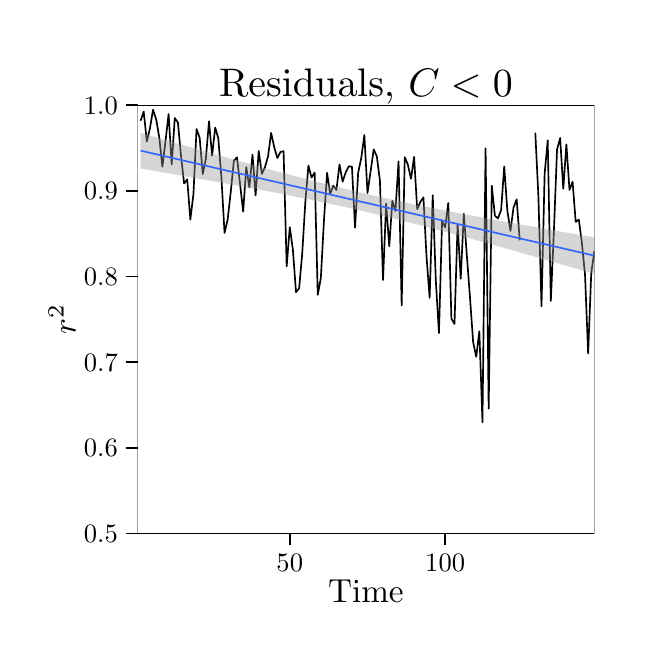
\begin{tikzpicture}[x=1pt,y=1pt]
\definecolor[named]{fillColor}{rgb}{1.00,1.00,1.00}
\path[use as bounding box,fill=fillColor,fill opacity=0.00] (0,0) rectangle (216.81,216.81);
\begin{scope}
\path[clip] (  0.00,  0.00) rectangle (216.81,216.81);
\definecolor[named]{drawColor}{rgb}{1.00,1.00,1.00}
\definecolor[named]{fillColor}{rgb}{1.00,1.00,1.00}

\path[draw=drawColor,line width= 0.6pt,line join=round,line cap=round,fill=fillColor] ( -0.00,  0.00) rectangle (216.81,216.81);
\end{scope}
\begin{scope}
\path[clip] ( 39.69, 34.03) rectangle (204.76,188.82);
\definecolor[named]{fillColor}{rgb}{1.00,1.00,1.00}

\path[fill=fillColor] ( 39.69, 34.03) rectangle (204.76,188.82);
\definecolor[named]{drawColor}{rgb}{0.00,0.00,0.00}

\path[draw=drawColor,line width= 0.6pt,line join=round] ( 40.81,183.17) --
	( 41.93,186.49) --
	( 43.06,175.66) --
	( 44.18,180.42) --
	( 45.30,187.13) --
	( 46.42,183.77) --
	( 47.55,177.15) --
	( 48.67,166.55) --
	( 49.79,175.68) --
	( 50.92,185.61) --
	( 52.04,167.40) --
	( 53.16,184.17) --
	( 54.29,182.51) --
	( 55.41,170.51) --
	( 56.53,160.51) --
	( 57.65,162.00) --
	( 58.78,147.46) --
	( 59.90,156.68) --
	( 61.02,180.17) --
	( 62.15,177.01) --
	( 63.27,163.89) --
	( 64.39,169.47) --
	( 65.52,182.96) --
	( 66.64,170.56) --
	( 67.76,180.73) --
	( 68.88,176.86) --
	( 70.01,162.68) --
	( 71.13,142.65) --
	( 72.25,147.38) --
	( 73.38,157.42) --
	( 74.50,168.69) --
	( 75.62,169.94) --
	( 76.74,160.37) --
	( 77.87,150.32) --
	( 78.99,166.42) --
	( 80.11,159.08) --
	( 81.24,170.92) --
	( 82.36,156.18) --
	( 83.48,172.24) --
	( 84.61,163.97) --
	( 85.73,166.36) --
	( 86.85,170.26) --
	( 87.97,178.79) --
	( 89.10,173.57) --
	( 90.22,169.72) --
	( 91.34,171.86) --
	( 92.47,172.18) --
	( 93.59,130.58) --
	( 94.71,144.74) --
	( 95.84,136.48) --
	( 96.96,121.23) --
	( 98.08,122.61) --
	( 99.20,135.07) --
	(100.33,153.80) --
	(101.45,166.96) --
	(102.57,162.65) --
	(103.70,164.43) --
	(104.82,120.25) --
	(105.94,126.37) --
	(107.07,147.27) --
	(108.19,164.36) --
	(109.31,156.71) --
	(110.43,159.75) --
	(111.56,158.15) --
	(112.68,167.38) --
	(113.80,161.15) --
	(114.93,164.55) --
	(116.05,166.72) --
	(117.17,166.59) --
	(118.30,144.53) --
	(119.42,164.36) --
	(120.54,169.70) --
	(121.66,178.02) --
	(122.79,157.05) --
	(123.91,164.83) --
	(125.03,172.80) --
	(126.16,170.32) --
	(127.28,161.59) --
	(128.40,125.62) --
	(129.53,153.25) --
	(130.65,137.81) --
	(131.77,154.24) --
	(132.89,150.54) --
	(134.02,168.51) --
	(135.14,116.42) --
	(136.26,170.02) --
	(137.39,167.28) --
	(138.51,162.21) --
	(139.63,170.10) --
	(140.75,151.26) --
	(141.88,153.77) --
	(143.00,155.51) --
	(144.12,134.13) --
	(145.25,119.13) --
	(146.37,156.27) --
	(147.49,125.19) --
	(148.62,106.43) --
	(149.74,146.81) --
	(150.86,144.70) --
	(151.98,153.44) --
	(153.11,111.66) --
	(154.23,109.76) --
	(155.35,145.84) --
	(156.48,126.08) --
	(157.60,149.54) --
	(158.72,134.15) --
	(159.85,119.05) --
	(160.97,103.15) --
	(162.09, 97.87) --
	(163.21,107.12) --
	(164.34, 74.21) --
	(165.46,173.21) --
	(166.58, 79.13) --
	(167.71,159.72) --
	(168.83,148.86) --
	(169.95,147.88) --
	(171.08,150.93) --
	(172.20,166.69) --
	(173.32,150.81) --
	(174.44,143.36) --
	(175.57,151.87) --
	(176.69,154.76) --
	(177.81,139.98);

\path[draw=drawColor,line width= 0.6pt,line join=round] (183.43,178.84) --
	(184.55,155.85) --
	(185.67,116.11) --
	(186.80,164.04) --
	(187.92,176.10) --
	(189.04,118.03) --
	(190.17,143.90) --
	(191.29,172.84) --
	(192.41,176.93) --
	(193.54,158.59) --
	(194.66,174.63) --
	(195.78,158.17) --
	(196.90,161.13) --
	(198.03,146.62) --
	(199.15,147.49) --
	(200.27,138.96) --
	(201.40,127.48) --
	(202.52, 99.08) --
	(203.64,128.05) --
	(204.76,136.04);
\definecolor[named]{fillColor}{rgb}{0.60,0.60,0.60}

\path[fill=fillColor,fill opacity=0.40] ( 40.81,178.82) --
	( 42.88,178.22) --
	( 44.96,177.61) --
	( 47.04,177.01) --
	( 49.11,176.41) --
	( 51.19,175.81) --
	( 53.26,175.22) --
	( 55.34,174.62) --
	( 57.41,174.02) --
	( 59.49,173.43) --
	( 61.56,172.83) --
	( 63.64,172.24) --
	( 65.71,171.65) --
	( 67.79,171.06) --
	( 69.86,170.48) --
	( 71.94,169.89) --
	( 74.02,169.31) --
	( 76.09,168.73) --
	( 78.17,168.15) --
	( 80.24,167.58) --
	( 82.32,167.00) --
	( 84.39,166.43) --
	( 86.47,165.87) --
	( 88.54,165.30) --
	( 90.62,164.74) --
	( 92.69,164.19) --
	( 94.77,163.63) --
	( 96.84,163.09) --
	( 98.92,162.54) --
	(101.00,162.00) --
	(103.07,161.47) --
	(105.15,160.94) --
	(107.22,160.41) --
	(109.30,159.90) --
	(111.37,159.38) --
	(113.45,158.87) --
	(115.52,158.37) --
	(117.60,157.88) --
	(119.67,157.39) --
	(121.75,156.91) --
	(123.82,156.43) --
	(125.90,155.96) --
	(127.98,155.50) --
	(130.05,155.04) --
	(132.13,154.58) --
	(134.20,154.14) --
	(136.28,153.70) --
	(138.35,153.26) --
	(140.43,152.83) --
	(142.50,152.41) --
	(144.58,151.99) --
	(146.65,151.57) --
	(148.73,151.16) --
	(150.80,150.75) --
	(152.88,150.35) --
	(154.96,149.95) --
	(157.03,149.55) --
	(159.11,149.16) --
	(161.18,148.77) --
	(163.26,148.38) --
	(165.33,148.00) --
	(167.41,147.62) --
	(169.48,147.24) --
	(171.56,146.86) --
	(173.63,146.48) --
	(175.71,146.11) --
	(177.78,145.74) --
	(179.86,145.37) --
	(181.94,145.00) --
	(184.01,144.63) --
	(186.09,144.27) --
	(188.16,143.90) --
	(190.24,143.54) --
	(192.31,143.18) --
	(194.39,142.82) --
	(196.46,142.46) --
	(198.54,142.10) --
	(200.61,141.74) --
	(202.69,141.38) --
	(204.76,141.03) --
	(204.76,127.84) --
	(202.69,128.45) --
	(200.61,129.05) --
	(198.54,129.65) --
	(196.46,130.25) --
	(194.39,130.85) --
	(192.31,131.45) --
	(190.24,132.05) --
	(188.16,132.65) --
	(186.09,133.24) --
	(184.01,133.84) --
	(181.94,134.43) --
	(179.86,135.02) --
	(177.78,135.61) --
	(175.71,136.20) --
	(173.63,136.79) --
	(171.56,137.37) --
	(169.48,137.96) --
	(167.41,138.54) --
	(165.33,139.12) --
	(163.26,139.69) --
	(161.18,140.27) --
	(159.11,140.84) --
	(157.03,141.40) --
	(154.96,141.97) --
	(152.88,142.53) --
	(150.80,143.09) --
	(148.73,143.64) --
	(146.65,144.19) --
	(144.58,144.73) --
	(142.50,145.27) --
	(140.43,145.81) --
	(138.35,146.34) --
	(136.28,146.86) --
	(134.20,147.38) --
	(132.13,147.90) --
	(130.05,148.41) --
	(127.98,148.91) --
	(125.90,149.41) --
	(123.82,149.90) --
	(121.75,150.38) --
	(119.67,150.86) --
	(117.60,151.33) --
	(115.52,151.79) --
	(113.45,152.25) --
	(111.37,152.71) --
	(109.30,153.15) --
	(107.22,153.59) --
	(105.15,154.03) --
	(103.07,154.46) --
	(101.00,154.89) --
	( 98.92,155.31) --
	( 96.84,155.72) --
	( 94.77,156.14) --
	( 92.69,156.54) --
	( 90.62,156.95) --
	( 88.54,157.35) --
	( 86.47,157.75) --
	( 84.39,158.14) --
	( 82.32,158.53) --
	( 80.24,158.92) --
	( 78.17,159.30) --
	( 76.09,159.68) --
	( 74.02,160.06) --
	( 71.94,160.44) --
	( 69.86,160.82) --
	( 67.79,161.19) --
	( 65.71,161.56) --
	( 63.64,161.94) --
	( 61.56,162.30) --
	( 59.49,162.67) --
	( 57.41,163.04) --
	( 55.34,163.40) --
	( 53.26,163.77) --
	( 51.19,164.13) --
	( 49.11,164.49) --
	( 47.04,164.85) --
	( 44.96,165.21) --
	( 42.88,165.57) --
	( 40.81,165.92) --
	cycle;
\definecolor[named]{drawColor}{rgb}{0.20,0.40,1.00}

\path[draw=drawColor,line width= 0.6pt,line join=round] ( 40.81,172.37) --
	( 42.88,171.89) --
	( 44.96,171.41) --
	( 47.04,170.93) --
	( 49.11,170.45) --
	( 51.19,169.97) --
	( 53.26,169.49) --
	( 55.34,169.01) --
	( 57.41,168.53) --
	( 59.49,168.05) --
	( 61.56,167.57) --
	( 63.64,167.09) --
	( 65.71,166.61) --
	( 67.79,166.13) --
	( 69.86,165.65) --
	( 71.94,165.17) --
	( 74.02,164.69) --
	( 76.09,164.21) --
	( 78.17,163.73) --
	( 80.24,163.25) --
	( 82.32,162.77) --
	( 84.39,162.29) --
	( 86.47,161.81) --
	( 88.54,161.33) --
	( 90.62,160.85) --
	( 92.69,160.37) --
	( 94.77,159.89) --
	( 96.84,159.41) --
	( 98.92,158.93) --
	(101.00,158.45) --
	(103.07,157.96) --
	(105.15,157.48) --
	(107.22,157.00) --
	(109.30,156.52) --
	(111.37,156.04) --
	(113.45,155.56) --
	(115.52,155.08) --
	(117.60,154.60) --
	(119.67,154.12) --
	(121.75,153.64) --
	(123.82,153.16) --
	(125.90,152.68) --
	(127.98,152.20) --
	(130.05,151.72) --
	(132.13,151.24) --
	(134.20,150.76) --
	(136.28,150.28) --
	(138.35,149.80) --
	(140.43,149.32) --
	(142.50,148.84) --
	(144.58,148.36) --
	(146.65,147.88) --
	(148.73,147.40) --
	(150.80,146.92) --
	(152.88,146.44) --
	(154.96,145.96) --
	(157.03,145.48) --
	(159.11,145.00) --
	(161.18,144.52) --
	(163.26,144.04) --
	(165.33,143.56) --
	(167.41,143.08) --
	(169.48,142.60) --
	(171.56,142.12) --
	(173.63,141.64) --
	(175.71,141.16) --
	(177.78,140.68) --
	(179.86,140.20) --
	(181.94,139.72) --
	(184.01,139.24) --
	(186.09,138.76) --
	(188.16,138.28) --
	(190.24,137.80) --
	(192.31,137.32) --
	(194.39,136.83) --
	(196.46,136.35) --
	(198.54,135.87) --
	(200.61,135.39) --
	(202.69,134.91) --
	(204.76,134.43);
\definecolor[named]{drawColor}{rgb}{0.00,0.00,0.00}

\path[draw=drawColor,line width= 0.6pt,line join=round,line cap=round] ( 39.69, 34.03) rectangle (204.76,188.82);
\end{scope}
\begin{scope}
\path[clip] (  0.00,  0.00) rectangle (216.81,216.81);
\definecolor[named]{drawColor}{rgb}{0.00,0.00,0.00}

\node[text=drawColor,anchor=base east,inner sep=0pt, outer sep=0pt, scale=  0.96] at ( 32.57, 30.73) {0.5};

\node[text=drawColor,anchor=base east,inner sep=0pt, outer sep=0pt, scale=  0.96] at ( 32.57, 61.69) {0.6};

\node[text=drawColor,anchor=base east,inner sep=0pt, outer sep=0pt, scale=  0.96] at ( 32.57, 92.64) {0.7};

\node[text=drawColor,anchor=base east,inner sep=0pt, outer sep=0pt, scale=  0.96] at ( 32.57,123.60) {0.8};

\node[text=drawColor,anchor=base east,inner sep=0pt, outer sep=0pt, scale=  0.96] at ( 32.57,154.56) {0.9};

\node[text=drawColor,anchor=base east,inner sep=0pt, outer sep=0pt, scale=  0.96] at ( 32.57,185.52) {1.0};
\end{scope}
\begin{scope}
\path[clip] (  0.00,  0.00) rectangle (216.81,216.81);
\definecolor[named]{drawColor}{rgb}{0.00,0.00,0.00}

\path[draw=drawColor,line width= 0.6pt,line join=round] ( 35.42, 34.03) --
	( 39.69, 34.03);

\path[draw=drawColor,line width= 0.6pt,line join=round] ( 35.42, 64.99) --
	( 39.69, 64.99);

\path[draw=drawColor,line width= 0.6pt,line join=round] ( 35.42, 95.95) --
	( 39.69, 95.95);

\path[draw=drawColor,line width= 0.6pt,line join=round] ( 35.42,126.91) --
	( 39.69,126.91);

\path[draw=drawColor,line width= 0.6pt,line join=round] ( 35.42,157.87) --
	( 39.69,157.87);

\path[draw=drawColor,line width= 0.6pt,line join=round] ( 35.42,188.82) --
	( 39.69,188.82);
\end{scope}
\begin{scope}
\path[clip] (  0.00,  0.00) rectangle (216.81,216.81);
\definecolor[named]{drawColor}{rgb}{0.00,0.00,0.00}

\path[draw=drawColor,line width= 0.6pt,line join=round] ( 94.71, 29.77) --
	( 94.71, 34.03);

\path[draw=drawColor,line width= 0.6pt,line join=round] (150.86, 29.77) --
	(150.86, 34.03);
\end{scope}
\begin{scope}
\path[clip] (  0.00,  0.00) rectangle (216.81,216.81);
\definecolor[named]{drawColor}{rgb}{0.00,0.00,0.00}

\node[text=drawColor,anchor=base,inner sep=0pt, outer sep=0pt, scale=  0.96] at ( 94.71, 20.31) {50};

\node[text=drawColor,anchor=base,inner sep=0pt, outer sep=0pt, scale=  0.96] at (150.86, 20.31) {100};
\end{scope}
\begin{scope}
\path[clip] (  0.00,  0.00) rectangle (216.81,216.81);
\definecolor[named]{drawColor}{rgb}{0.00,0.00,0.00}

\node[text=drawColor,anchor=base,inner sep=0pt, outer sep=0pt, scale=  1.20] at (122.23,  9.03) {Time};
\end{scope}
\begin{scope}
\path[clip] (  0.00,  0.00) rectangle (216.81,216.81);
\definecolor[named]{drawColor}{rgb}{0.00,0.00,0.00}

\node[text=drawColor,rotate= 90.00,anchor=base,inner sep=0pt, outer sep=0pt, scale=  1.20] at ( 17.30,111.43) {$r^2$};
\end{scope}
\begin{scope}
\path[clip] (  0.00,  0.00) rectangle (216.81,216.81);
\definecolor[named]{drawColor}{rgb}{0.00,0.00,0.00}

\node[text=drawColor,anchor=base,inner sep=0pt, outer sep=0pt, scale=  1.44] at (122.23,191.84) {Residuals, $C<0$};
\end{scope}
\end{tikzpicture}

\end{figure}
\begin{figure}
\centering
% Created by tikzDevice version 0.7.0 on 2015-04-30 12:06:26
% !TEX encoding = UTF-8 Unicode
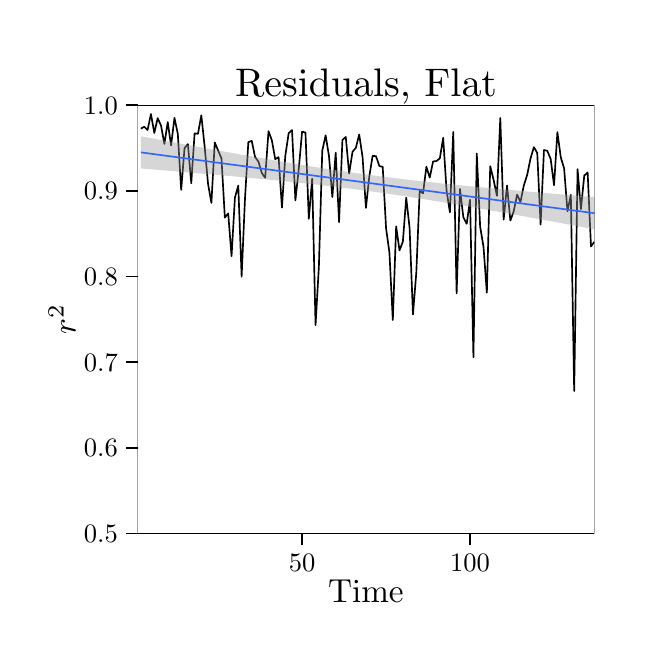
\begin{tikzpicture}[x=1pt,y=1pt]
\definecolor[named]{fillColor}{rgb}{1.00,1.00,1.00}
\path[use as bounding box,fill=fillColor,fill opacity=0.00] (0,0) rectangle (216.81,216.81);
\begin{scope}
\path[clip] (  0.00,  0.00) rectangle (216.81,216.81);
\definecolor[named]{drawColor}{rgb}{1.00,1.00,1.00}
\definecolor[named]{fillColor}{rgb}{1.00,1.00,1.00}

\path[draw=drawColor,line width= 0.6pt,line join=round,line cap=round,fill=fillColor] ( -0.00,  0.00) rectangle (216.81,216.81);
\end{scope}
\begin{scope}
\path[clip] ( 39.69, 34.03) rectangle (204.76,188.82);
\definecolor[named]{fillColor}{rgb}{1.00,1.00,1.00}

\path[fill=fillColor] ( 39.69, 34.03) rectangle (204.76,188.82);
\definecolor[named]{drawColor}{rgb}{0.00,0.00,0.00}

\path[draw=drawColor,line width= 0.6pt,line join=round] ( 40.90,180.32) --
	( 42.11,181.01) --
	( 43.33,179.84) --
	( 44.54,185.59) --
	( 45.76,178.77) --
	( 46.97,184.11) --
	( 48.18,181.47) --
	( 49.40,174.79) --
	( 50.61,182.69) --
	( 51.82,174.25) --
	( 53.04,184.21) --
	( 54.25,178.44) --
	( 55.47,158.20) --
	( 56.68,173.27) --
	( 57.89,174.74) --
	( 59.11,160.62) --
	( 60.32,178.61) --
	( 61.54,178.47) --
	( 62.75,185.16) --
	( 63.96,173.72) --
	( 65.18,160.37) --
	( 66.39,153.47) --
	( 67.60,175.32) --
	( 68.82,172.45) --
	( 70.03,169.57) --
	( 71.25,148.17) --
	( 72.46,149.70) --
	( 73.67,134.24) --
	( 74.89,155.39) --
	( 76.10,159.73) --
	( 77.31,126.83) --
	( 78.53,155.13) --
	( 79.74,175.44) --
	( 80.96,175.90) --
	( 82.17,170.06) --
	( 83.38,168.41) --
	( 84.60,164.32) --
	( 85.81,162.56) --
	( 87.03,179.42) --
	( 88.24,176.09) --
	( 89.45,169.29) --
	( 90.67,170.03) --
	( 91.88,151.79) --
	( 93.09,170.49) --
	( 94.31,178.67) --
	( 95.52,179.81) --
	( 96.74,154.43) --
	( 97.95,165.66) --
	( 99.16,179.26) --
	(100.38,178.89) --
	(101.59,147.74) --
	(102.80,162.25) --
	(104.02,109.30) --
	(105.23,130.54) --
	(106.45,172.33) --
	(107.66,177.91) --
	(108.87,170.50) --
	(110.09,155.60) --
	(111.30,171.61) --
	(112.52,146.52) --
	(113.73,176.22) --
	(114.94,177.32) --
	(116.16,164.09) --
	(117.37,171.93) --
	(118.58,173.40) --
	(119.80,178.20) --
	(121.01,170.04) --
	(122.23,151.68) --
	(123.44,163.05) --
	(124.65,170.51) --
	(125.87,170.36) --
	(127.08,166.80) --
	(128.29,166.51) --
	(129.51,144.28) --
	(130.72,135.49) --
	(131.94,111.16) --
	(133.15,144.98) --
	(134.36,136.32) --
	(135.58,139.52) --
	(136.79,155.40) --
	(138.01,144.34) --
	(139.22,113.18) --
	(140.43,128.28) --
	(141.65,157.84) --
	(142.86,156.95) --
	(144.07,166.56) --
	(145.29,162.63) --
	(146.50,168.48) --
	(147.72,168.62) --
	(148.93,169.56) --
	(150.14,177.03) --
	(151.36,158.00) --
	(152.57,150.04) --
	(153.78,179.14) --
	(155.00,120.75) --
	(156.21,158.52) --
	(157.43,148.29) --
	(158.64,145.94) --
	(159.85,154.60) --
	(161.07, 97.70) --
	(162.28,171.32) --
	(163.50,144.89) --
	(164.71,137.66) --
	(165.92,121.03) --
	(167.14,166.74) --
	(168.35,161.86) --
	(169.56,156.05) --
	(170.78,184.19) --
	(171.99,147.44) --
	(173.21,159.79) --
	(174.42,147.12) --
	(175.63,150.46) --
	(176.85,156.47) --
	(178.06,153.80) --
	(179.27,159.75) --
	(180.49,163.59) --
	(181.70,169.54) --
	(182.92,173.64) --
	(184.13,171.56) --
	(185.34,145.65) --
	(186.56,172.60) --
	(187.77,172.30) --
	(188.99,169.34) --
	(190.20,159.87) --
	(191.41,179.04) --
	(192.63,169.98) --
	(193.84,165.96) --
	(195.05,150.48) --
	(196.27,156.39) --
	(197.48, 85.51) --
	(198.70,165.70) --
	(199.91,151.23) --
	(201.12,163.35) --
	(202.34,164.52) --
	(203.55,137.75) --
	(204.76,139.42);
\definecolor[named]{fillColor}{rgb}{0.60,0.60,0.60}

\path[fill=fillColor,fill opacity=0.40] ( 40.90,177.57) --
	( 42.97,177.18) --
	( 45.05,176.80) --
	( 47.12,176.41) --
	( 49.20,176.03) --
	( 51.27,175.64) --
	( 53.35,175.26) --
	( 55.42,174.87) --
	( 57.49,174.49) --
	( 59.57,174.11) --
	( 61.64,173.73) --
	( 63.72,173.35) --
	( 65.79,172.98) --
	( 67.87,172.60) --
	( 69.94,172.23) --
	( 72.01,171.86) --
	( 74.09,171.49) --
	( 76.16,171.12) --
	( 78.24,170.75) --
	( 80.31,170.39) --
	( 82.39,170.02) --
	( 84.46,169.67) --
	( 86.53,169.31) --
	( 88.61,168.95) --
	( 90.68,168.60) --
	( 92.76,168.26) --
	( 94.83,167.91) --
	( 96.90,167.57) --
	( 98.98,167.23) --
	(101.05,166.90) --
	(103.13,166.57) --
	(105.20,166.25) --
	(107.28,165.93) --
	(109.35,165.61) --
	(111.42,165.30) --
	(113.50,164.99) --
	(115.57,164.69) --
	(117.65,164.40) --
	(119.72,164.11) --
	(121.80,163.83) --
	(123.87,163.55) --
	(125.94,163.28) --
	(128.02,163.01) --
	(130.09,162.75) --
	(132.17,162.49) --
	(134.24,162.24) --
	(136.32,161.99) --
	(138.39,161.75) --
	(140.46,161.52) --
	(142.54,161.28) --
	(144.61,161.06) --
	(146.69,160.83) --
	(148.76,160.61) --
	(150.83,160.40) --
	(152.91,160.19) --
	(154.98,159.98) --
	(157.06,159.77) --
	(159.13,159.57) --
	(161.21,159.37) --
	(163.28,159.17) --
	(165.35,158.98) --
	(167.43,158.79) --
	(169.50,158.60) --
	(171.58,158.41) --
	(173.65,158.22) --
	(175.73,158.04) --
	(177.80,157.86) --
	(179.87,157.67) --
	(181.95,157.49) --
	(184.02,157.32) --
	(186.10,157.14) --
	(188.17,156.96) --
	(190.25,156.79) --
	(192.32,156.61) --
	(194.39,156.44) --
	(196.47,156.27) --
	(198.54,156.10) --
	(200.62,155.93) --
	(202.69,155.76) --
	(204.76,155.59) --
	(204.76,143.94) --
	(202.69,144.33) --
	(200.62,144.72) --
	(198.54,145.11) --
	(196.47,145.49) --
	(194.39,145.88) --
	(192.32,146.26) --
	(190.25,146.64) --
	(188.17,147.03) --
	(186.10,147.41) --
	(184.02,147.79) --
	(181.95,148.16) --
	(179.87,148.54) --
	(177.80,148.92) --
	(175.73,149.29) --
	(173.65,149.66) --
	(171.58,150.03) --
	(169.50,150.40) --
	(167.43,150.77) --
	(165.35,151.13) --
	(163.28,151.49) --
	(161.21,151.85) --
	(159.13,152.21) --
	(157.06,152.56) --
	(154.98,152.91) --
	(152.91,153.26) --
	(150.83,153.61) --
	(148.76,153.95) --
	(146.69,154.28) --
	(144.61,154.62) --
	(142.54,154.95) --
	(140.46,155.27) --
	(138.39,155.59) --
	(136.32,155.91) --
	(134.24,156.22) --
	(132.17,156.52) --
	(130.09,156.82) --
	(128.02,157.12) --
	(125.94,157.41) --
	(123.87,157.69) --
	(121.80,157.97) --
	(119.72,158.24) --
	(117.65,158.51) --
	(115.57,158.77) --
	(113.50,159.03) --
	(111.42,159.28) --
	(109.35,159.52) --
	(107.28,159.77) --
	(105.20,160.00) --
	(103.13,160.23) --
	(101.05,160.46) --
	( 98.98,160.68) --
	( 96.90,160.90) --
	( 94.83,161.12) --
	( 92.76,161.33) --
	( 90.68,161.54) --
	( 88.61,161.74) --
	( 86.53,161.95) --
	( 84.46,162.15) --
	( 82.39,162.34) --
	( 80.31,162.54) --
	( 78.24,162.73) --
	( 76.16,162.92) --
	( 74.09,163.11) --
	( 72.01,163.29) --
	( 69.94,163.48) --
	( 67.87,163.66) --
	( 65.79,163.84) --
	( 63.72,164.02) --
	( 61.64,164.20) --
	( 59.57,164.38) --
	( 57.49,164.55) --
	( 55.42,164.73) --
	( 53.35,164.90) --
	( 51.27,165.08) --
	( 49.20,165.25) --
	( 47.12,165.42) --
	( 45.05,165.59) --
	( 42.97,165.76) --
	( 40.90,165.93) --
	cycle;
\definecolor[named]{drawColor}{rgb}{0.20,0.40,1.00}

\path[draw=drawColor,line width= 0.6pt,line join=round] ( 40.90,171.75) --
	( 42.97,171.47) --
	( 45.05,171.19) --
	( 47.12,170.91) --
	( 49.20,170.64) --
	( 51.27,170.36) --
	( 53.35,170.08) --
	( 55.42,169.80) --
	( 57.49,169.52) --
	( 59.57,169.24) --
	( 61.64,168.97) --
	( 63.72,168.69) --
	( 65.79,168.41) --
	( 67.87,168.13) --
	( 69.94,167.85) --
	( 72.01,167.58) --
	( 74.09,167.30) --
	( 76.16,167.02) --
	( 78.24,166.74) --
	( 80.31,166.46) --
	( 82.39,166.18) --
	( 84.46,165.91) --
	( 86.53,165.63) --
	( 88.61,165.35) --
	( 90.68,165.07) --
	( 92.76,164.79) --
	( 94.83,164.51) --
	( 96.90,164.24) --
	( 98.98,163.96) --
	(101.05,163.68) --
	(103.13,163.40) --
	(105.20,163.12) --
	(107.28,162.85) --
	(109.35,162.57) --
	(111.42,162.29) --
	(113.50,162.01) --
	(115.57,161.73) --
	(117.65,161.45) --
	(119.72,161.18) --
	(121.80,160.90) --
	(123.87,160.62) --
	(125.94,160.34) --
	(128.02,160.06) --
	(130.09,159.78) --
	(132.17,159.51) --
	(134.24,159.23) --
	(136.32,158.95) --
	(138.39,158.67) --
	(140.46,158.39) --
	(142.54,158.12) --
	(144.61,157.84) --
	(146.69,157.56) --
	(148.76,157.28) --
	(150.83,157.00) --
	(152.91,156.72) --
	(154.98,156.45) --
	(157.06,156.17) --
	(159.13,155.89) --
	(161.21,155.61) --
	(163.28,155.33) --
	(165.35,155.05) --
	(167.43,154.78) --
	(169.50,154.50) --
	(171.58,154.22) --
	(173.65,153.94) --
	(175.73,153.66) --
	(177.80,153.39) --
	(179.87,153.11) --
	(181.95,152.83) --
	(184.02,152.55) --
	(186.10,152.27) --
	(188.17,151.99) --
	(190.25,151.72) --
	(192.32,151.44) --
	(194.39,151.16) --
	(196.47,150.88) --
	(198.54,150.60) --
	(200.62,150.32) --
	(202.69,150.05) --
	(204.76,149.77);
\definecolor[named]{drawColor}{rgb}{0.00,0.00,0.00}

\path[draw=drawColor,line width= 0.6pt,line join=round,line cap=round] ( 39.69, 34.03) rectangle (204.76,188.82);
\end{scope}
\begin{scope}
\path[clip] (  0.00,  0.00) rectangle (216.81,216.81);
\definecolor[named]{drawColor}{rgb}{0.00,0.00,0.00}

\node[text=drawColor,anchor=base east,inner sep=0pt, outer sep=0pt, scale=  0.96] at ( 32.57, 30.73) {0.5};

\node[text=drawColor,anchor=base east,inner sep=0pt, outer sep=0pt, scale=  0.96] at ( 32.57, 61.69) {0.6};

\node[text=drawColor,anchor=base east,inner sep=0pt, outer sep=0pt, scale=  0.96] at ( 32.57, 92.64) {0.7};

\node[text=drawColor,anchor=base east,inner sep=0pt, outer sep=0pt, scale=  0.96] at ( 32.57,123.60) {0.8};

\node[text=drawColor,anchor=base east,inner sep=0pt, outer sep=0pt, scale=  0.96] at ( 32.57,154.56) {0.9};

\node[text=drawColor,anchor=base east,inner sep=0pt, outer sep=0pt, scale=  0.96] at ( 32.57,185.52) {1.0};
\end{scope}
\begin{scope}
\path[clip] (  0.00,  0.00) rectangle (216.81,216.81);
\definecolor[named]{drawColor}{rgb}{0.00,0.00,0.00}

\path[draw=drawColor,line width= 0.6pt,line join=round] ( 35.42, 34.03) --
	( 39.69, 34.03);

\path[draw=drawColor,line width= 0.6pt,line join=round] ( 35.42, 64.99) --
	( 39.69, 64.99);

\path[draw=drawColor,line width= 0.6pt,line join=round] ( 35.42, 95.95) --
	( 39.69, 95.95);

\path[draw=drawColor,line width= 0.6pt,line join=round] ( 35.42,126.91) --
	( 39.69,126.91);

\path[draw=drawColor,line width= 0.6pt,line join=round] ( 35.42,157.87) --
	( 39.69,157.87);

\path[draw=drawColor,line width= 0.6pt,line join=round] ( 35.42,188.82) --
	( 39.69,188.82);
\end{scope}
\begin{scope}
\path[clip] (  0.00,  0.00) rectangle (216.81,216.81);
\definecolor[named]{drawColor}{rgb}{0.00,0.00,0.00}

\path[draw=drawColor,line width= 0.6pt,line join=round] ( 99.16, 29.77) --
	( 99.16, 34.03);

\path[draw=drawColor,line width= 0.6pt,line join=round] (159.85, 29.77) --
	(159.85, 34.03);
\end{scope}
\begin{scope}
\path[clip] (  0.00,  0.00) rectangle (216.81,216.81);
\definecolor[named]{drawColor}{rgb}{0.00,0.00,0.00}

\node[text=drawColor,anchor=base,inner sep=0pt, outer sep=0pt, scale=  0.96] at ( 99.16, 20.31) {50};

\node[text=drawColor,anchor=base,inner sep=0pt, outer sep=0pt, scale=  0.96] at (159.85, 20.31) {100};
\end{scope}
\begin{scope}
\path[clip] (  0.00,  0.00) rectangle (216.81,216.81);
\definecolor[named]{drawColor}{rgb}{0.00,0.00,0.00}

\node[text=drawColor,anchor=base,inner sep=0pt, outer sep=0pt, scale=  1.20] at (122.23,  9.03) {Time};
\end{scope}
\begin{scope}
\path[clip] (  0.00,  0.00) rectangle (216.81,216.81);
\definecolor[named]{drawColor}{rgb}{0.00,0.00,0.00}

\node[text=drawColor,rotate= 90.00,anchor=base,inner sep=0pt, outer sep=0pt, scale=  1.20] at ( 17.30,111.43) {$r^2$};
\end{scope}
\begin{scope}
\path[clip] (  0.00,  0.00) rectangle (216.81,216.81);
\definecolor[named]{drawColor}{rgb}{0.00,0.00,0.00}

\node[text=drawColor,anchor=base,inner sep=0pt, outer sep=0pt, scale=  1.44] at (122.23,191.84) {Residuals, Flat};
\end{scope}
\end{tikzpicture}

\end{figure}
\end{document}